\chapter{Interacciones con el blanco}

Esta clase tiene como objetivo familiarizarnos con la interpretación visual de imágenes SAR en las bandas L, C y X. Para esto se estudiaran las interacciones con distintos blancos para cada una de las bandas.

\section{Interpretación visual}

Para las imágenes radar hay 3 grandes grupos de interacciones posibles entre el blanco: doble rebote, en volumen y especular. Como será esta interacción va a depender tanto del blanco como de la banda en la que funciona el satélite (Figura \ref{fig:interacciones})

\begin{figure}[h!]
    \centering
    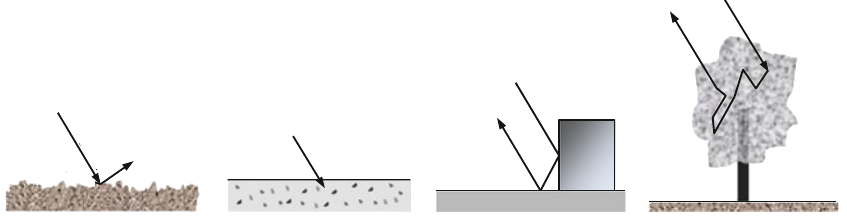
\includegraphics[width=0.5\textwidth]{fig:interacciones.png}
    \caption{Interacciónes con distintos blancos: -a- superficial, -b- subsuperficial, -c- doble rebote y -d- en volumen.}
    \label{fig:interacciones}
\end{figure}

\subsection{Banda-X}

Las imágenes adquiridas en \emph{Banda X} son las que tienen menor longitud de onda. Serán por lo tanto las que menos penetración tengan en la vegetación y las que más componente de backscatter presenten en suelos sin cobertura (Figura \ref{fig:interacciones}).


Abra la imagen \path{CSKS3_GEC_B_S2_03_HH_RD_SF_20141221211655_20141221211703.h5} de la carpeta \path{material/raster_data/COSMO}. Despliege la banda \path{Sigma_HH_db}.

Observe guiandose con la imagen óptica:

\begin{enumerate}
    \item En que color se observa la pista de aterrizaje.
    \item En que color se ven las zonas urbanas.
    \item En que color se observan las zonas con vegetación.
    \item En que color se observa el agua que está en el lago.
    \item En que color se observa el agua del canal.
\end{enumerate}

\begin{que}
    ¿Que le permite decir sobre la geometría de cada blanco los valores de backscatter encontrados arriba?
\end{que}

\subsection{Banda C}

Las imágenes adquiridas en \emph{Banda C} son las que tienen longitudes de onda intermedias. Tendrán por lo tanto menos reflectancia en los suelos sin coberturaa y nos permitiran extraer información sobre el scattering en volumnes (Figura \ref{fig:interacciones}).

Abra la imagen \path{SENTINEL} de la carpeta \path{material/raster_data/SENTINEL1}. Despliege la banda \path{Sigma_HH_db}.

Observe guiandose con la imagen óptica:

\begin{enumerate}
    \item En que color se observa la pista de aterrizaje.
    \item En que color se ven las zonas urbanas.
    \item En que color se observan las zonas con vegetación.
    \item En que color se observa el agua que está en el lago.
    \item En que color se observa el agua del canal.
\end{enumerate}

\begin{que}
    ¿Que le permite decir sobre la geometría de cada blanco los valores de backscatter encontrados arriba?
\end{que}
\subsection{Banda L}

Las imágenes adquiridas en \emph{Banda L} son las que tienen mayor longitud de onda. Tendran en general interacciones especulares con los suelos sin cobertura, pero una buena longitud de penetración en la superficie. Además permitirán identificar propiedades de las coberturas vegetadas por debajo del canopeo (Figura \ref{fig:interacciones}).

Abra la imagen \path{ALOS} de la carpeta \path{material/raster_data/ALOS}. Despliege la banda \path{Sigma_HH_db}.


Observe guiandose con la imagen óptica:

\begin{enumerate}
    \item En que color se observa la pista de aterrizaje.
    \item En que color se ven las zonas urbanas.
    \item En que color se observan las zonas con vegetación.
    \item En que color se observa el agua que está en el lago.
    \item En que color se observa el agua del canal.
\end{enumerate}

\begin{que}
    ¿Que le permite decir sobre la geometría de cada blanco los valores de backscatter encontrados arriba?
\end{que}

\section{Valores de $dB$}

Es habitual expresar el valor del coeficiente de backscatter en dB para las imágenes SAR. Para calcularlo en distintos sectores de la imagen puede posicionarse sobre un píxel y observar en \emph{Pixel info} el valor de \path{Sigma0_HH_db} en dB.

Observe guiandose con la imagen óptica para la imagen \path{COSMO}:

\begin{enumerate}
    \item Cuanto vale el valor de dB para la pista de aterrizaje.
    \item Cuanto vale el valor de dB para las zonas urbanas.
    \item Cuanto vale el valor de dB para las zonas con vegetación.
    \item Cuanto vale el valor de dB para el agua que está en el lago.
    \item Cuanto vale el valor de dB para el agua del canal.
\end{enumerate}

Otra forma de obtener estos valores es calculando el promedio sobre una región. Para esto haga click en \emph{Vector, New Vector Data Container} y ponga el nombre \emph{Úrbano} (Figura \ref{fig:vector-cont}). Seleccione luego la herramienta \emph{Rectangle drawing tool} de la barra de herramienta y digitalice un rectangulo sobre la zona úrbana. Para confirmar la geometría haga click fuera de ella luego de crearla

\begin{figure}[h!]
    \centering
    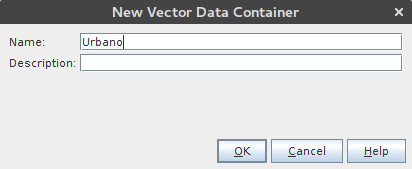
\includegraphics[scale=0.4]{fig:vector-cont.png}
    \caption{}
    \label{fig:vector-cont}
\end{figure}

Repita el proceso y cree contenedores de vectores para zonas de vegetación, agua con alto y bajo brillo y la pista de aterrizaje.

Dirijase luego al menú \emph{Analysis, Statistics} y en la ventana que aparece tilde la opción \emph{Use ROI maks(s)} (Figura \ref{fig:estadistica}). Seleccione la región Urbano y haga click en el botón \emph{Refresh view}. El SNAP calculará la estadística para la zona y devolverá la estadística para la región seleccionada. Puede seleccionar varias regiones en simultaneo para calcular la estadística en cada una.

\begin{figure}[h!]
    \centering
    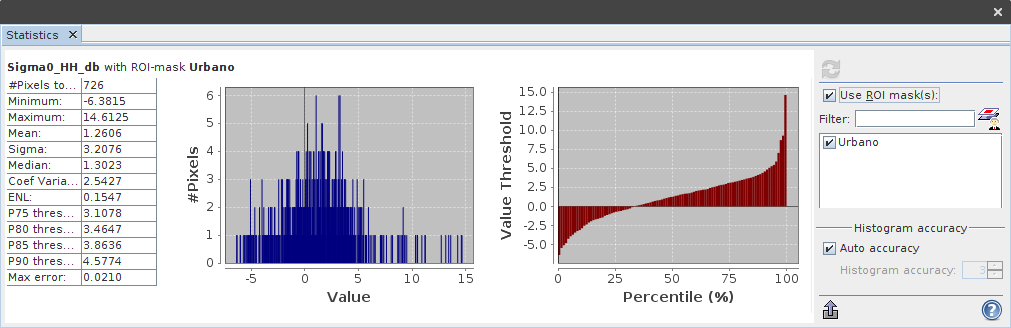
\includegraphics[scale=0.4]{fig:estadistica.png}
    \caption{}
    \label{fig:estadistica}
\end{figure}

Repita este analisis para las imágenes en banda L y C.

\section{Actividad}

Comparando las tres imágenes SAR utilizadas responda

\begin{que}
    ¿Que coberturas tienen siempre valores altos de brillo? ¿Como se puede interpretar geometricamente?
\end{que}

\begin{que}
    ¿Que coberturas tienen siempre valores bajos de brillo? ¿Como se puede interpretar geometricamente?
\end{que}

\begin{que}
    ¿Cual es la cobertura que más cambian al cambiar de una banda a otra?
\end{que}

\begin{que}
    ¿Cuales son las coberturas con más ruido dentro de las imágenes?
\end{que}

\begin{que}
    Observe las imágenes que no se encuentran en dB. ¿Que diferencia encuentra en la distribución de valores de brillo?
\end{que}
